In this section, we demonstrate the beampatterns obtained from Algorithm \ref{alg:A} and \ref{alg:B} 
and the baselines in both LOS-dominated Rician channel and Rayleigh channel.

Figure \ref{fig:beampattern_rayleigh_single_fully} compares the averaged beampattern from Monte-Carlo simulation when BS-RIS and RIS-user channels follow 
Rayleigh fading ($\varepsilon = 0$).
One can visualize from Figure \ref{fig:beampattern_rayleigh_single_fully_a} and \ref{fig:beampattern_rayleigh_single_fully_c} that both single connected and fully connected RIS make tiny improvement to the beampattern 
compared with baseline when the WSR is small. However, as shown in Figure \ref{fig:beampattern_rayleigh_single_fully_b} and \ref{fig:beampattern_rayleigh_single_fully_d}, when WSR increases to a large value, i.e., $5.4$bps/Hz and $7.9$bps/Hz, fully connected 
RIS achieves the largest probing power at target. The gains achieved by fully connected RIS in separated deployment 
over single connected RIS and baseline are 2.2dB and 4.7dB, respectively. The counterparts in shared deployment are 2.7dB and 4.8dB.

\begin{figure}[ht]
    \centering
    \subfigure[Separated deployment: WSR = $1.0$bps/Hz]{
        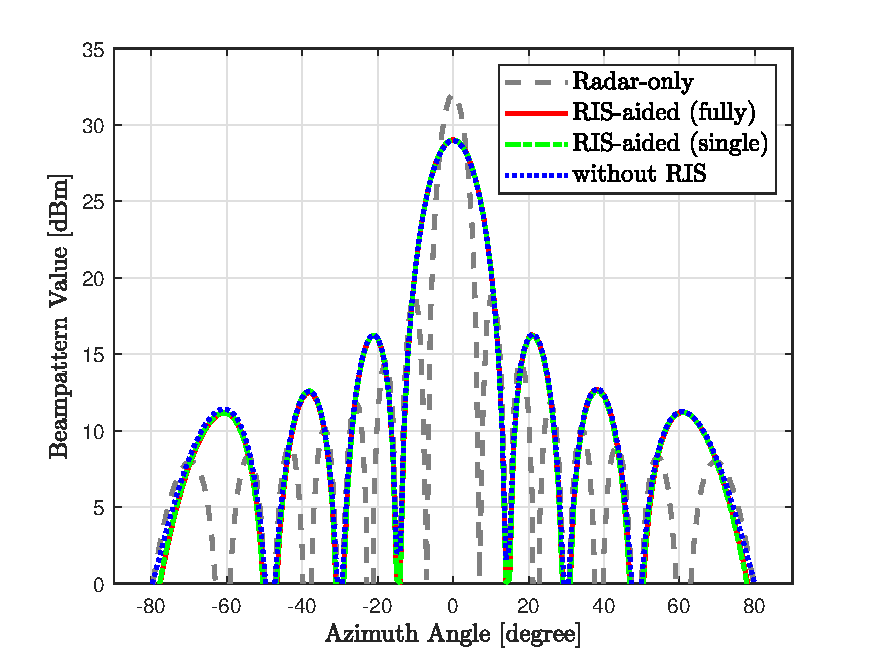
\includegraphics[width=0.475\textwidth]{beampattern_rayleigh_single_fully_a.pdf}
        \label{fig:beampattern_rayleigh_single_fully_a}
    }
    \subfigure[Separated deployment: WSR = $5.4$bps/Hz]{
	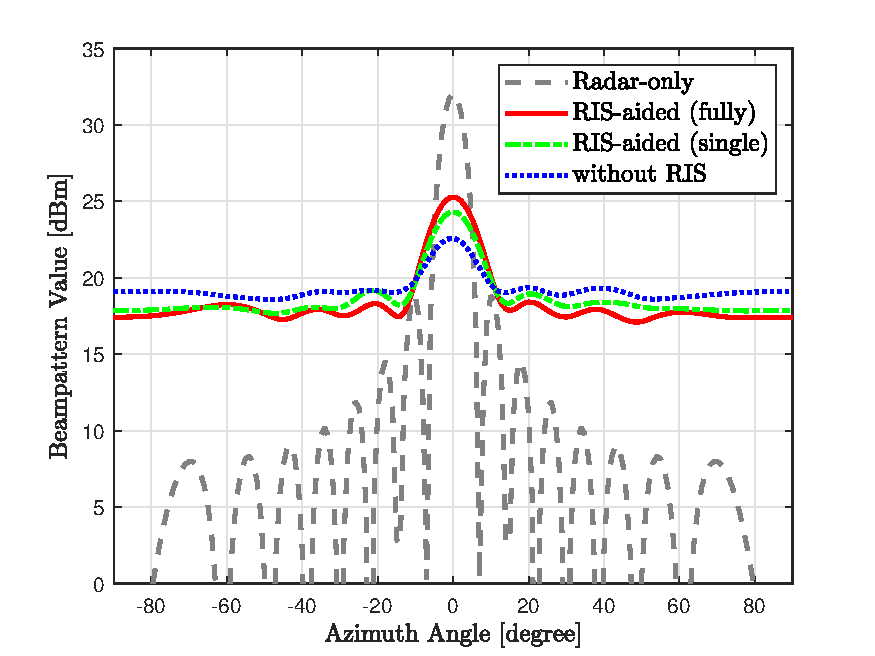
\includegraphics[width=0.475\textwidth]{beampattern_rayleigh_single_fully_b.pdf}
        \label{fig:beampattern_rayleigh_single_fully_b}
    }

    \subfigure[Shared deployment: WSR = $1.8$bps/Hz]{
        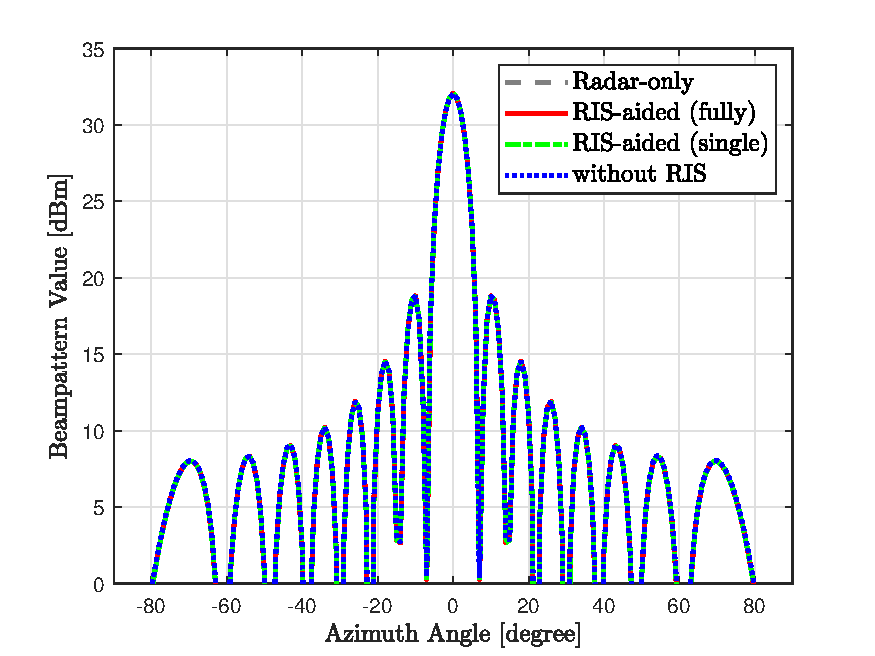
\includegraphics[width=0.475\textwidth]{beampattern_rayleigh_single_fully_c.pdf}
        \label{fig:beampattern_rayleigh_single_fully_c}
    }
    \subfigure[Shared deployment: WSR = $7.9$bps/Hz]{
	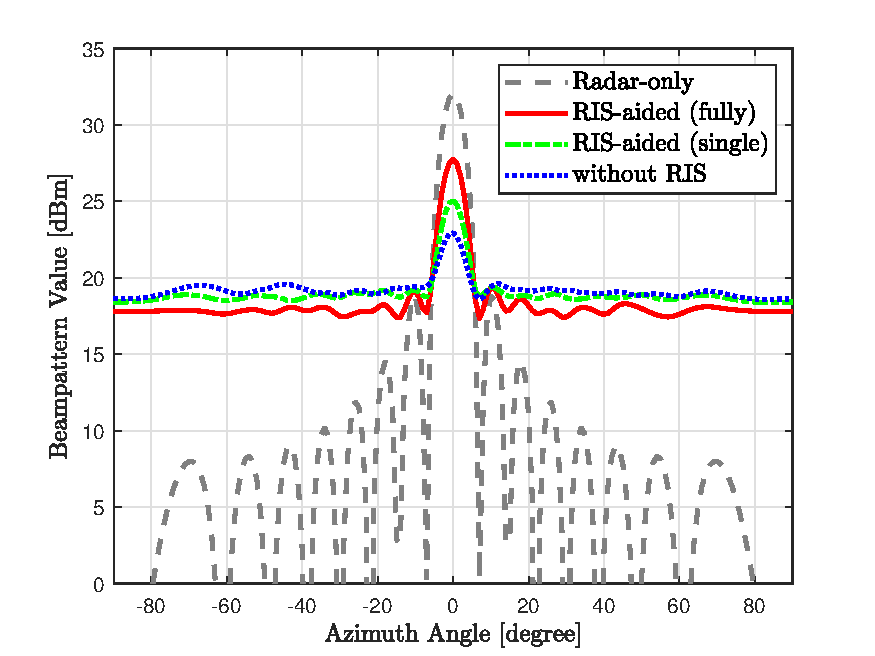
\includegraphics[width=0.475\textwidth]{beampattern_rayleigh_single_fully_d.pdf}
        \label{fig:beampattern_rayleigh_single_fully_d}
    }
    \caption{Beampattern comparison in Rayleigh channel ($\varepsilon = 0$)}
    \label{fig:beampattern_rayleigh_single_fully}
\end{figure}

Figure \ref{fig:beampattern_los_single_fully} compares the averaged beampattern when the BS-RIS and RIS-user channels are LOS-dominated  Rician channel ($\varepsilon = 1000$). 
We can see that in both separated and shared deployment the fully connected RIS does not outperform the single connected RIS significantly in terms of probing power no matter the 
WSR is large or small. Therefore, the fully connected only shows advantages when the BS-RIS and RIS-user channels follow Rayleigh fading.
The scaling law in \cite{shen2020modeling} indicates that the fully connected and single connected RIS achieves the same 
received power at users in LOS channel because the model of LOS channel leads to the same optimal ${\bf \Theta}$. This scaling law
can also explain the results in Figure \ref{fig:beampattern_los_single_fully}: the model of LOS channel also leads to the same optimal ${\bf \Theta}$ in terms of WSR, 
so that the WSR is the same when the probing power at target is the same. 

\begin{figure}[ht]
    \centering
    \subfigure[Separated deployment: WSR = $1.0$bps/Hz]{
        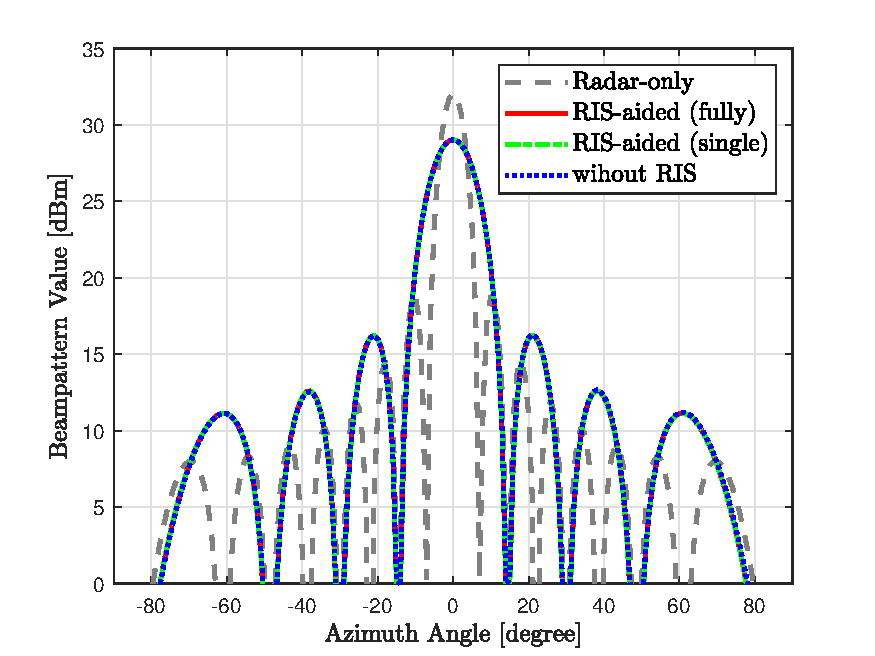
\includegraphics[width=0.475\textwidth]{beampattern_los_single_fully_a.pdf}
        \label{fig:beampattern_los_single_fully_a}
    }
    \subfigure[Separated deployment: WSR = $5.4$bps/Hz]{
    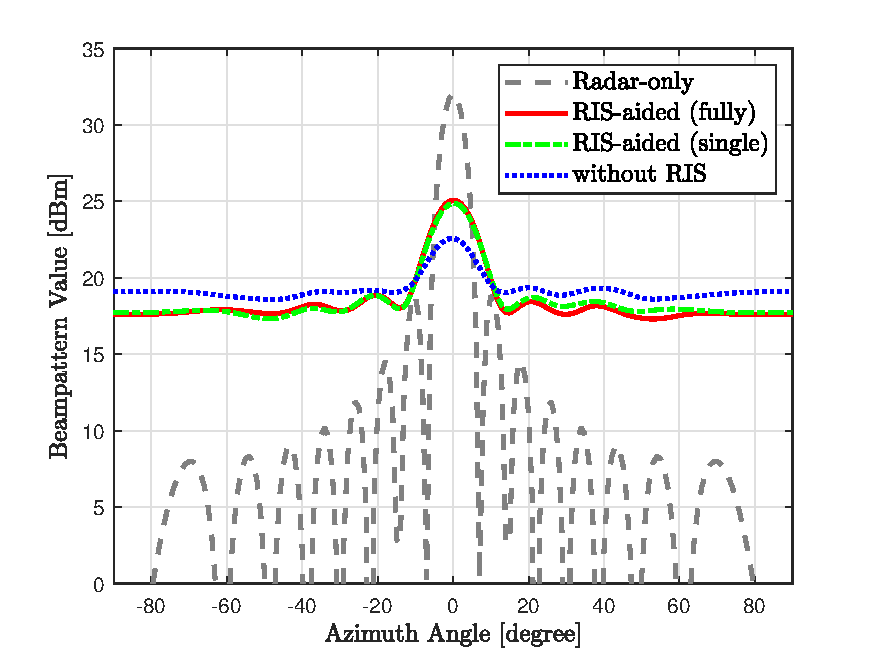
\includegraphics[width=0.475\textwidth]{beampattern_los_single_fully_b.pdf}
        \label{fig:beampattern_los_single_fully_b}
    }

    \subfigure[Shared deployment: WSR = $1.8$bps/Hz]{
        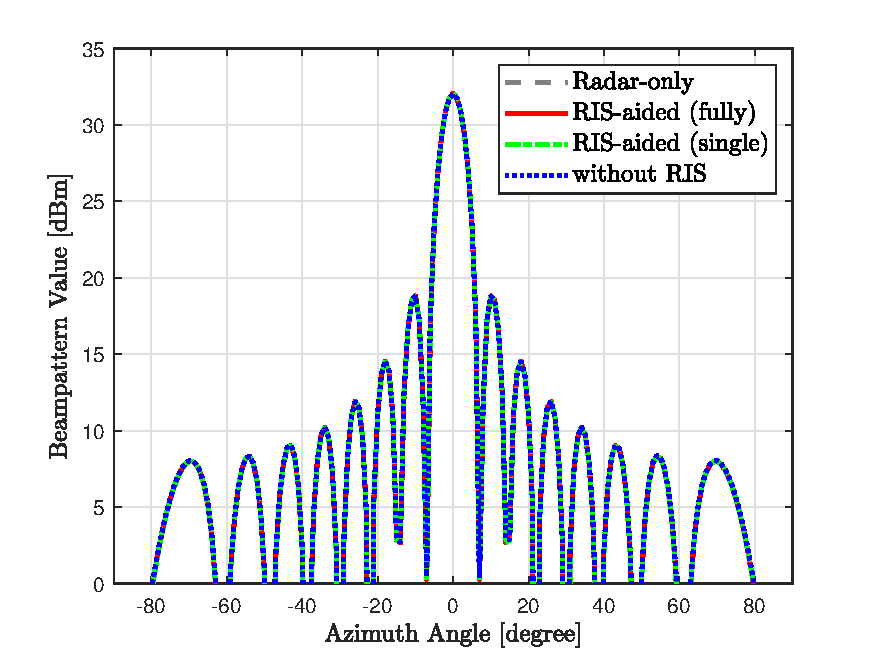
\includegraphics[width=0.475\textwidth]{beampattern_los_single_fully_c.pdf}
        \label{fig:beampattern_los_single_fully_c}
    }
    \subfigure[Shared deployment: WSR = $7.9$bps/Hz]{
    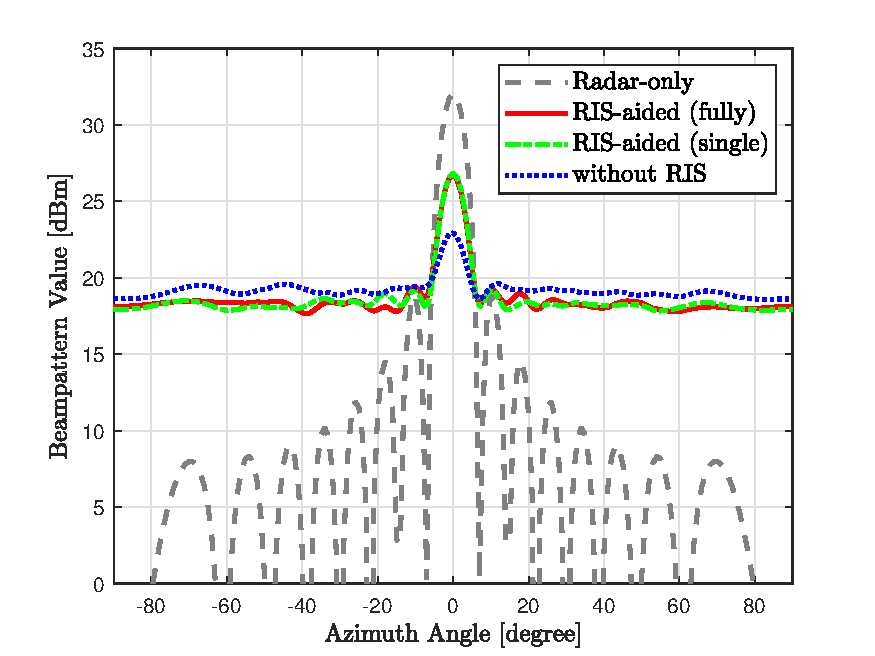
\includegraphics[width=0.475\textwidth]{beampattern_los_single_fully_d.pdf}
        \label{fig:beampattern_los_single_fully_d}
    }
    \caption{Beampattern comparison in LOS-dominated  Rician channel ($\varepsilon = 1000$)}
    \label{fig:beampattern_los_single_fully}
\end{figure}



Figure \ref{fig:beampattern_reflecting_elements} shows the effect of the number of reflecting elements in LOS-dominated  Rician channel. As the fully connected and 
single connected RIS perform the same in LOS channel, only single connected RIS is considered in Figure \ref{fig:beampattern_reflecting_elements}. We can see that 
the better beampattern and higher probing power at target are achieved as the growth of element amounts. Nevertheless, the improvement
is not to infinity but asymptotically reaches an upper bound. For example, in shared deployment, the probing power at target increases by
4.9dB as the reflecting element increases from 0 to 20, while the gains are reduced to 1.2dB and 0.2dB when the amount changes from 20 to 60 and from 60 to 100,
respectively.

Figure \ref{fig:beampattern_rayleigh_separated_shared} compares the beampattern of separated and shared deployments. It displays that the mainlobe of beampattern
in shared deployment is much more narrow than that in separated deployment, which is more directional. With the help of RIS,
the probing power at target in shared deployment is only $0.13$dB lower than the Radar-only system when there are 100 reflecting elements.

\begin{figure}
	\centering
	\begin{minipage}[t]{1\linewidth}
        \centering
        \subfigure[Separated deployment: WSR = $5.4$bps/Hz]{
        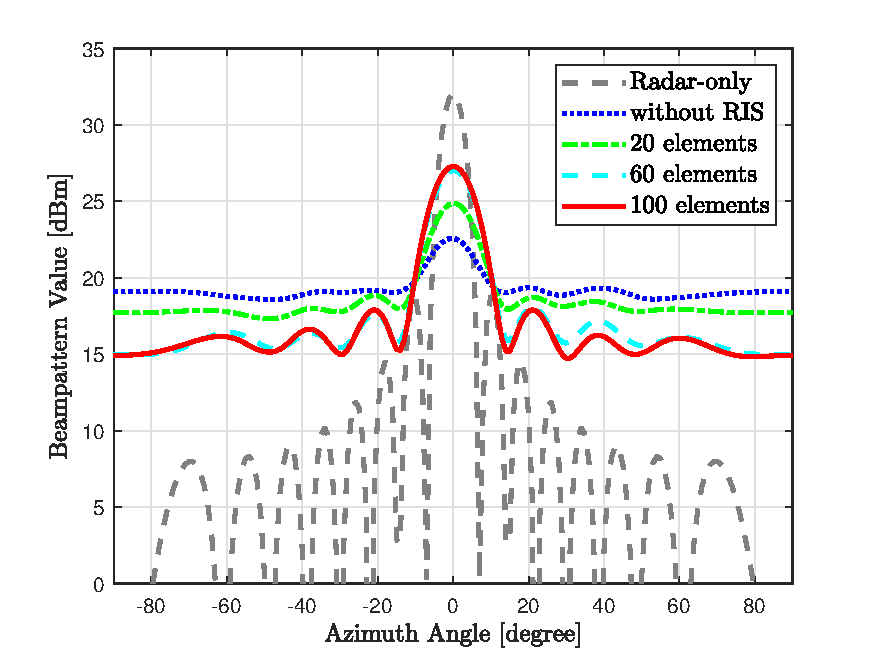
\includegraphics[width=0.475\textwidth]{beampattern_reflecting_elements_a.pdf}
            \label{fig:beampattern_reflecting_elements_a}
        }
        \subfigure[Shared deployment: WSR = $7.9$bps/Hz]{
        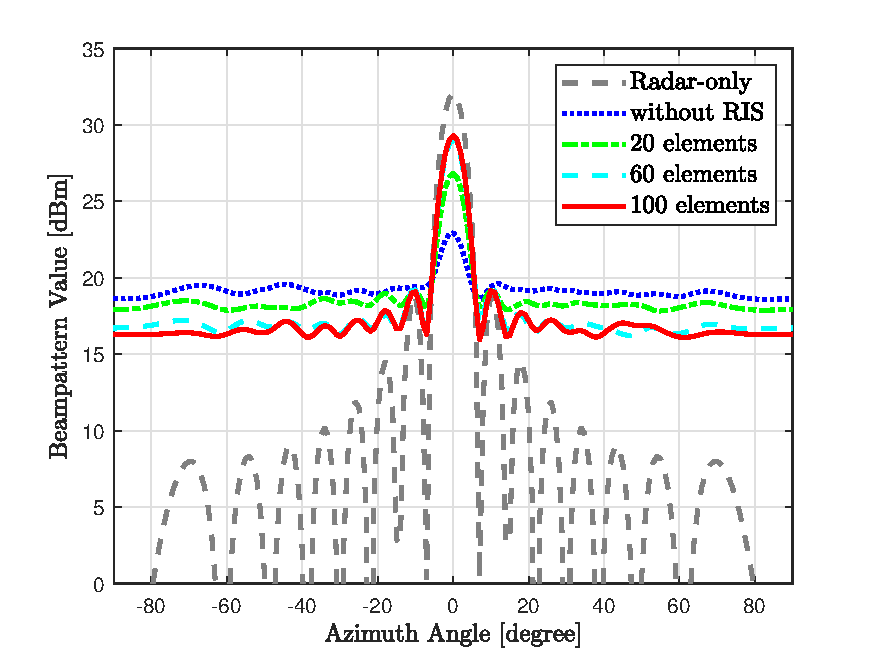
\includegraphics[width=0.475\textwidth]{beampattern_reflecting_elements_b.pdf}
            \label{fig:beampattern_reflecting_elements_b}
        }
        \caption{Effect of the number of reflecting elements on beampattern in LOS-dominated Rician channel}
        \label{fig:beampattern_reflecting_elements}
	\end{minipage}
	\\
	\begin{minipage}[t]{1\linewidth}
        \centering
        \subfigure[without RIS, WSR = $5.4$bps/Hz]{
            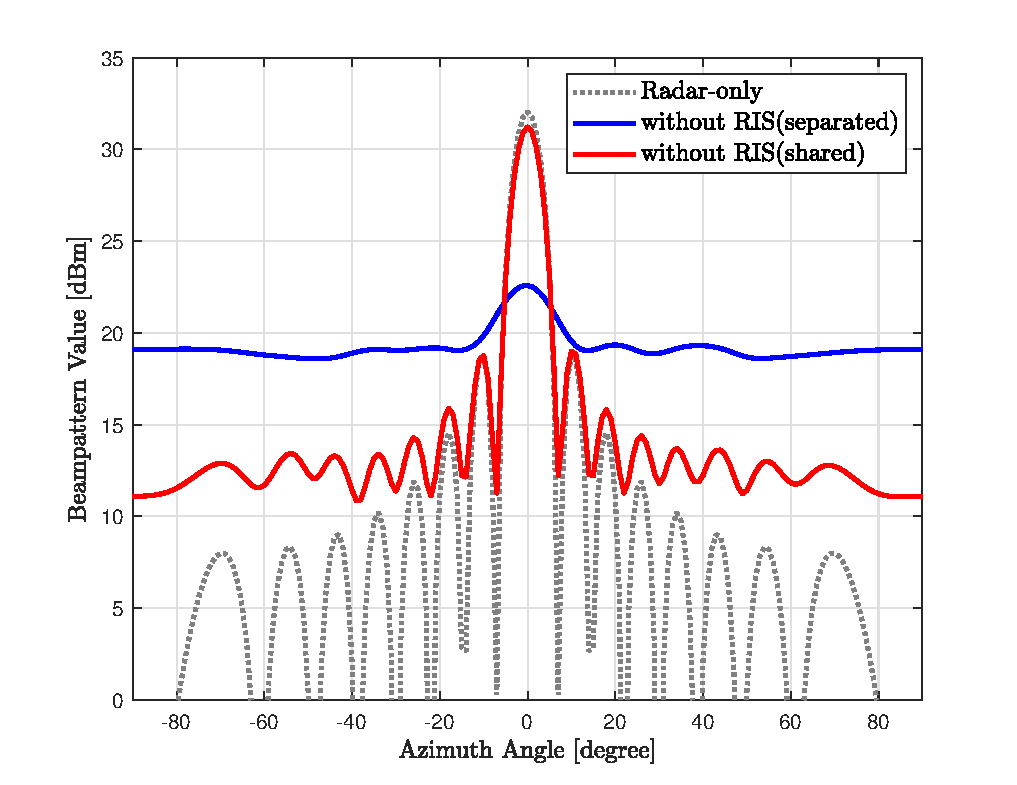
\includegraphics[width=0.475\textwidth]{beampattern_rayleigh_separated_shared_a.pdf}
            \label{fig:beampattern_rayleigh_separated_shared_a}
        }
        \subfigure[20 elements, WSR = $5.4$bps/Hz]{
        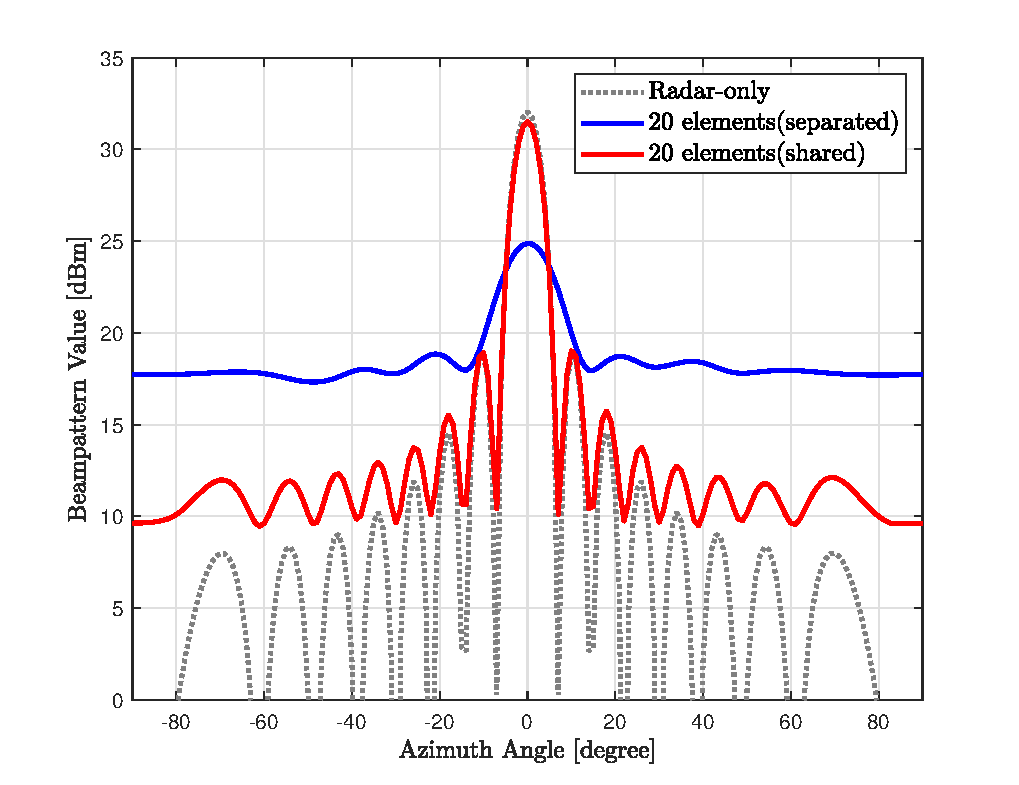
\includegraphics[width=0.475\textwidth]{beampattern_rayleigh_separated_shared_b.pdf}
            \label{fig:beampattern_rayleigh_separated_shared_b}
        }
    
        \subfigure[60 elements, WSR = $5.4$bps/Hz]{
            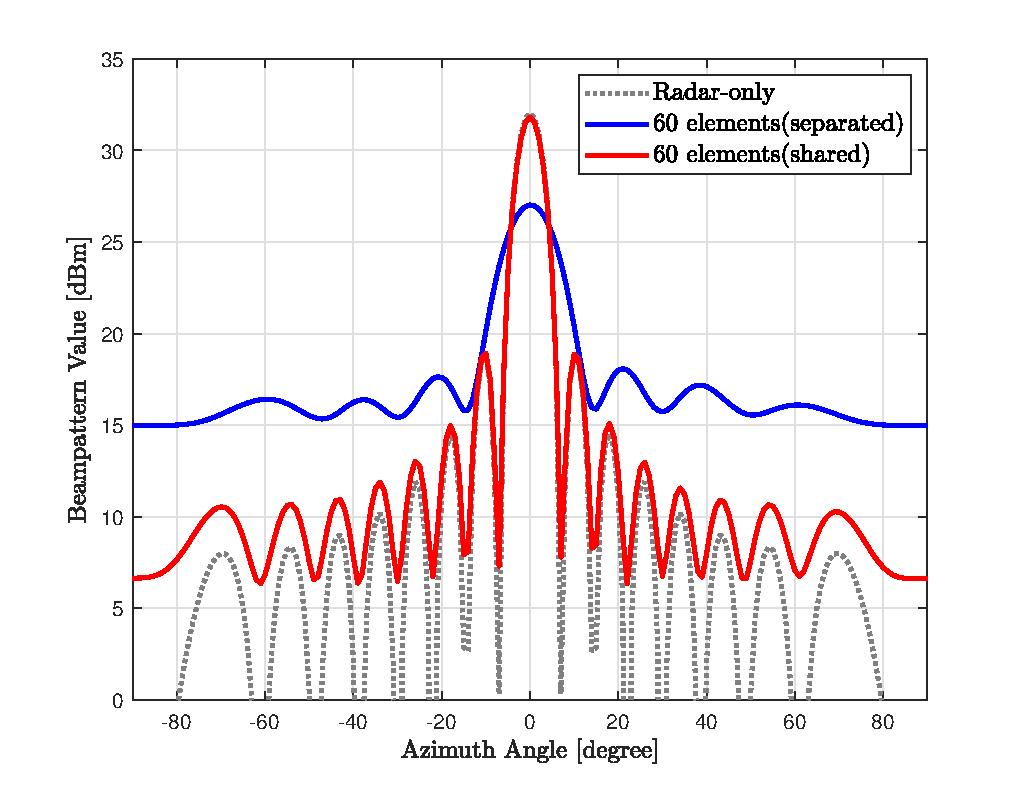
\includegraphics[width=0.475\textwidth]{beampattern_rayleigh_separated_shared_c.pdf}
            \label{fig:beampattern_rayleigh_separated_shared_c}
        }
        \subfigure[100 elements, WSR = $5.4$bps/Hz]{
        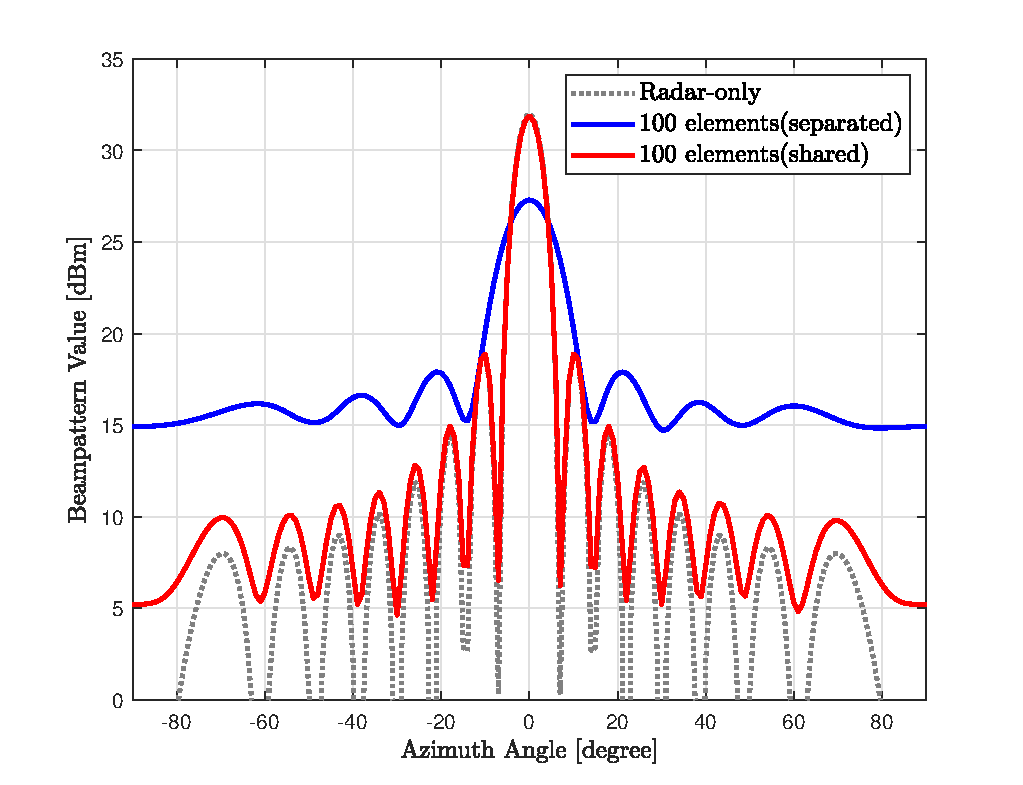
\includegraphics[width=0.475\textwidth]{beampattern_rayleigh_separated_shared_d.pdf}
            \label{fig:beampattern_rayleigh_separated_shared_d}
        }
        \caption{Beampattern comparison of separated and share deployment in LOS-dominated Rician channel}
        \label{fig:beampattern_rayleigh_separated_shared}
	\end{minipage}
\end{figure}